% cloned from https://gitlab.kit.edu/kit/kastel/sdq/dokumentvorlagen/praesentationen/beamer
% commit: df83435a0d7e4308ba4115901166d32237c94d67

\documentclass[en, navbarinline, handout]{sdqbeamer}
% remove animation roll-out: handout (general "beamer" option, not specific for this class)
% layout options: 16:9 (default), 16:10, 4:3
% footer font size options: bigfoot (default), smallfoot (KIT layout)
% navigation bar options: navbarinline (default), navbarinfooter, navbarside, navbaroff, navbarkit (off + smallfoot)
% language: de (default), en

\titleimage{title_image}

\grouplogo{}

\groupname{PhD Defense}
%\groupnamewidth{50mm} % default

\title[Leveraging Constraints for User-Centric Feature Selection]{Leveraging Constraints for User-Centric Feature Selection} % [footer]{title slide}
\subtitle{PhD Defense}
\author[Jakob Bach]{Jakob Bach} % [footer]{title slide}

\date[2025-01-20]{January 20, 2025} % [footer]{title slide}

%\usepackage{amsmath} % mathematical symbols and equations; apparently pre-loaded
%\usepackage{amssymb} % mathematical symbols; apparently pre-loaded
\usepackage[style=numeric, backend=biber]{biblatex}
\usepackage{booktabs} % nicely formatted tables (with top, mid, and bottom rule)
%\usepackage{graphicx} % plots; apparently pre-loaded
\usepackage[font=normalsize]{subcaption} % subfigures
\usepackage{tikz} % used for non-float figure positioning
%\usepackage{hyperref} % links and URLs; apparently pre-loaded

\addbibresource{references.bib}

\hypersetup{colorlinks=true, citecolor=kit-blue, linkcolor=kit-blue, urlcolor=kit-blue}

\setlength{\leftmargini}{0.2cm} % change default indentation (so items are left-aligned to boxes)
\setlength{\leftmarginii}{0.3cm} % 2nd level indentation
\setlength{\leftmarginiii}{0.3cm} % 3rd level indentation

\setbeamerfont{itemize/enumerate subsubbody}{size=\small} % make 3rd-level items as large as 2nd-level ones (default is \footnotesize, as defined in "beamerfontthemedefault.sty")

\setbeamercovered{invisible} % use "transparent" to show later content of animated slide in gray

\renewcommand{\textcite}[1]{\citeauthor{#1} (\citeyear{#1}) \cite{#1}}  % we generally have numeric style, but want longer citations on one slide; \textcite only shows author name(s) for our citation style, so we redefine it to "<<Author(s)>> (<<year>>) [<<ref>>]"

\begin{document}

\KITtitleframe

\section{Introduction}

\begin{frame}[t]{Background}
	%JB: want to clarify which scenario we talk about
	%JB: very generally, we are in field of data science / machine learning, want to make predictions
	\begin{definition}[Feature selection]
		\pause
		Given a dataset~$X \in \mathbb{R}^{m \times n}$
		with prediction target~$y \in Y^m$ (e.g., $Y = \mathbb{R}$ or $Y = \{0, 1\}$),\\
		\pause
		\emph{feature selection} is the problem of making feature-selection decisions~$s \in \{0,1\}^n$\\
		\pause
		that maximize a given notion of feature-set quality~$Q(s,X,y)$.\\
		\pause
		Typically, select a fixed number of features~$k \in \mathbb{N}$, i.e., $\sum_{j=1}^n s_j = k$.
	\end{definition}
	%JB: tabular data, where rows are data objects ("m" is their number) and columns are features ("n" is their number)
	%JB: supervised scenario
	%JB: examples for prediction target from our experiments (though our methods are domain-independent): is person credit-worthy? is e-mail spam? is mushroom poisonous? will horse survive illness?
	%JB: feature engineering already done (e.g., in spam example)
	%JB: different white-box and black-box objectives for quality, depending on feature-selection method (from correlating each feature with the target to running a genetic algorithm wrapped around a prediction model)
	\pause
	\vspace{-0.5\baselineskip}
	\begin{columns}
		\column[t]{0.50\textwidth}
		\begin{itemize}
			\item Reasons for feature selection~\cite{chandrashekar2014survey, li2017feature}:
			\begin{itemize}
				\item Increase interpretability of predictions
				%JB: most important reason for us (matches theme of user-centricity)
				%JB: prediction models with less features tend to be more interpretable but also depends on model
				\item Reduce computational requirements of machine learning (CPU, memory, storage, power consumption)
				%JB: requirements for training and prediction
				\item Improve prediction performance
				%JB: has been argued in literature, but IMHO questionable since you throw away information
				%JB: some models better if irrelevant or misleading information removed beforehand
			\end{itemize}
		\end{itemize}
		\column[t]{0.46\textwidth}
		\pause[2] % show table together with first part of definition
		\vspace{-0.5\baselineskip}
		\begin{table}
			\begin{tabular}{cccccc}
				\cmidrule(lr){1-4} \cmidrule(lr){6-6}
				Feat\_1 & Feat\_2 & \dots & Feat\_$n$ & \quad & Target \\
				\cmidrule(lr){1-4} \cmidrule(lr){6-6}
				$X_{11}$ & $X_{12}$ & \dots & $X_{1n}$ & & $y_1$ \\
				$X_{21}$ & $X_{22}$ & \dots & $X_{2n}$ & & $y_2$ \\
				\dots & \dots & \dots & \dots & & \dots \\
				$X_{m1}$ & $X_{m2}$ & \dots & $X_{mn}$ & & $y_m$ \\
				\cmidrule(lr){1-4} \cmidrule(lr){6-6}
			\end{tabular}
		\end{table}
	\end{columns}
*\end{frame}

\begin{frame}[t]{Motivation and Our Approach}
	\begin{itemize}
		\item Main limitations of most existing feature-selection methods:
		\begin{itemize}
			\item Do not consider domain knowledge
			%JB: Q() is a technical criterion, and there are typically no constraints apart from cardinality
			%JB: technically good feature sets may still be hard to interpret if they don't make sense from domain perspective
			%JB: e.g., domain experts may say that if certain feature selected, another should be selected as well, or two features should NOT be selected simultaneously
			%JB: domain knowledge may be firm, hypotheses, preferences
			%JB: in literature, there are at most approaches integrating specific constraint types into specific FS methods (apart from the work of Groves)
			\item Return only one feature set, no alternatives
			%JB: may be misleading if there are alternative solutions with similar quality
			%JB: e.g., if domain experts derive hypotheses about domain from selected features
		\end{itemize}
		\pause
		\vspace{\baselineskip}
		\item Central idea of dissertation: Make feature selection more user-centric via constraints
		%JB: we use constraints in propositional logic and linear arithmetic
		\begin{itemize}
			\item Still optimize feature-set quality but restrict valid feature selections
			\item Formulate as white-box optimization problem and use solver
		\end{itemize}
		\pause
		%
		\begin{example}[A feature-selection constraint in propositional logic]
			$(\lnot s_1 \land \lnot s_2 \land \lnot s_3) \lor (s_1 \land s_2 \land s_3) \leftrightarrow$ ``Select none or all of Features 1, 2, and 3.''
		\end{example}
		%JB: that formulation is rather general; more specific: scientific study and several features together characterize an underlying qunatity/mechanism, so either all or none should be selected
		%
		\pause
		\vspace{0.2\baselineskip}
		\item Benefits of our approach:
		\begin{itemize}
			\item Declarative
			\item Allows combining constraints
			\item Orthogonal to choice of feature-selection method
			%JB: related work typically integrates one constraint type into one feature-selection method
			%JB: feature-selection method determines objective, our constraints are independent of objective
			%JB: solver accepts a broad range of constraints and there are general way to combine solver with objective
		\end{itemize}
	\end{itemize}
\end{frame}

\begin{frame}[t]{Our Contributions}
	\vspace{-\baselineskip} % \columns seems to add vertical whitespace
	%JB: four core contributions, correspond to four chapters in main part of dissertation
	%JB: will discuss these to varying degree (due to limited time)
	\begin{columns}
		\column[t]{0.55\textwidth}
		\begin{itemize}
			\item (C1) Evaluating the impact of constraints \cite{bach2022empirical}
			\begin{itemize}
				\item Formalize constrained feature selection
				%JB: general framework on which later work builds
				\item Domain-independent study on impact of constraints
				%JB: more on that later
			\end{itemize}
			\item (C2) Using constraints to formulate scientific hypotheses \cite{bach2022empirical}
			\begin{itemize}
				\item Domain-specific study on impact of constraints
				%JB: in materials science (will not be discussed in detail); worked with domain experts to formulate constraints
			\end{itemize}
			%JB: worked on (C1) and (C2) in parallel (same formalization, but experiments domain- independent vs. specific), joint publication
			\pause
			\item (C3) Using constraints for alternative feature sets \cite{bach2023finding, bach2024alternative}
			\begin{itemize}
				\item Formalize alternative feature selection
				\item Discuss integrating constraints
				%JB: into feature-selection methods
				\item Analyze time complexity
				\item Propose heuristic search methods
				%JB: besides solver-based search
				\item Experimental study
			\end{itemize}
			%JB: now focus on a specific, domain-independent constraint type
			%JB: second publication (with journal and arXiv version)
		\end{itemize}
		\pause
		\column[t]{0.41\textwidth}
		\begin{itemize}
			\item (C4) Using constraints for feature selection in subgroup discovery \cite{bach2025subgroup, bach2024using}
			%JB: we will discuss subgroup discovery later; can be seen as an extension of feature selection
			\begin{itemize}
				\item Formalize subgroup-discovery as SMT optimization problem
				\item Formalize two constraint types
				\item Discuss integrating constraints
				\item Analyze time complexity
				\item Experimental study
			\end{itemize}
			%JB: can see some similarity: formalization, analysis, experiments
			%JB: again, specific constraint types
			%JB: third publication (with confererence and arXiv version)
			\pause
			\item Reproducibility:
			%JB: more a meta-contribution
			\begin{itemize}
				\item All experimental data available on \href{https://doi.org/10.35097/4kjyeg0z2bxmr6eh}{RADAR4KIT}
				\item Three GitHub repositories [\href{https://github.com/Jakob-Bach/Constrained-Filter-Feature-Selection}{a}, \href{https://github.com/Jakob-Bach/Alternative-Feature-Selection}{b}, \href{https://github.com/Jakob-Bach/Constrained-Subgroup-Discovery}{c}]
				\item Three Python packages: \href{https://pypi.org/project/alfese/}{\texttt{alfese}}, \href{https://pypi.org/project/cffs/}{\texttt{cffs}}, \href{https://pypi.org/project/csd/}{\texttt{csd}}
			\end{itemize}
		\end{itemize}
	\end{columns}
\end{frame}

\section{Constrained Feature Selection}

\begin{frame}[t]{(C1) Evaluating the Impacts of Constraints -- Approach}
	%JB: after general overview of our work, now deeper into a concrete contribution
	\begin{itemize}
		\item Systematic study on impact of constraints on feature-selection results
		\begin{itemize}
			\item Metrics for constraints, e.g, fraction of valid feature sets
			%JB: 4 metrics: number of constraints, number of (unique) constrained features, fraction of valid feature sets
			\item Metrics for results, e.g, feature-set quality
			%JB: 3 metrics: number of selected features, objective value, prediction performance
		\end{itemize}
		\pause
		\vspace{\baselineskip}
		\item Experimental design:
		\begin{itemize}
			\item 35 regression datasets from \emph{OpenML}~\cite{vanschoren2014openml}
			%JB: solution counting is expensive, therefore low dimensionality (10-14 features)
			%JB: 10-fold cross-validation
			\item Linear objective: $Q(s,X,y) = \sum_{j=1}^{n} q(X_{\cdot{}j},y) \cdot s_j$ (using mutual information~\cite{kraskov2004estimating} as $q(\cdot)$)
			%JB: very simple notion of feature-set quality (univariate filter)
			%JB: absolute Pearson correlation yielded similar insights
			%JB: also train four prediction models trained with selected features afterwards, but not in presented results: linear regression, regression tree, boosted linear model, boosted trees~\cite{chen2016xgboost, pedregosa2011scikit}
			\item Generate random constraints for ten constraint types with 1000 repetitions
			%JB: in each repetition, randomly choose features (for a varying number of constraints)
			%JB: unconstrained base case also is one of the constraint types
			\item \emph{Z3}~\cite{bjorner2015nuz, deMoura2008z3} (an SMT solver) as optimizer
			%JB: SMT = Satisfiablity Modulo Theories: generalizes propositional logic (in our case, with linear arithmetic) (other explanation: first-order logic but with specific interpretations of functions and predicates)
		\end{itemize}
	\end{itemize}
	\pause
	\vspace{0.5\baselineskip}
	\begin{examples}[Constraint types]
		\setlength{\leftmargini}{0.4cm} % box is aligned with slide's itemize, so we need not move items in box a bit to right (setting only applies locally)
		\begin{itemize}
			\item $\text{Single-XOR}(s_{j_1}, s_{j_2}) = s_{j_1} \oplus s_{j_2} = (s_{j_1} \land \lnot s_{j_2}) \lor (\lnot s_{j_1} \land s_{j_2})$
			% JB; some constraints relate to only two features ("single"), some to a group of features ("group"), some to all ("global")
			\item $\text{Group-NAND}(\{s_{j_1}, \dots, s_{j_{n'}}\}) =	\lnot (s_{j_1} \land s_{j_2} \land \dots \land s_{j_{n'}}) = \sum_{l=1}^{n'} s_{j_l} \leq n'-1$
		\end{itemize}
	\end{examples}
\end{frame}

\begin{frame}[t]{(C1) Evaluating the Impacts of Constraints -- Results}
	\begin{figure}
		\centering
		\begin{subfigure}{0.48\textwidth}
			\centering
			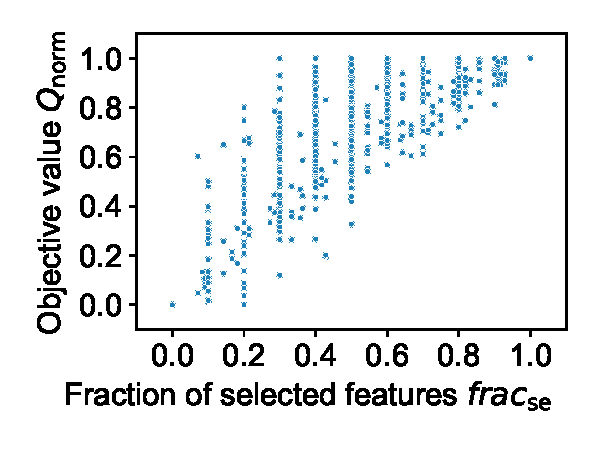
\includegraphics[width=0.95\textwidth, trim={0 15 0 10}, clip]{plots/syn-selected-vs-objective.pdf}
			%JB: all experimental results downsampled to 1000 random results to control plot file size
			%JB: normalization of number of selected features: divide by number of features in dataset
			%JB: normalization of objective value: divide by summed quality of all features of dataset
			%JB: clear correlation between number of selected features and objective (is expected)
		\end{subfigure}
		\hfill
		\begin{subfigure}{0.48\textwidth}
			\centering
			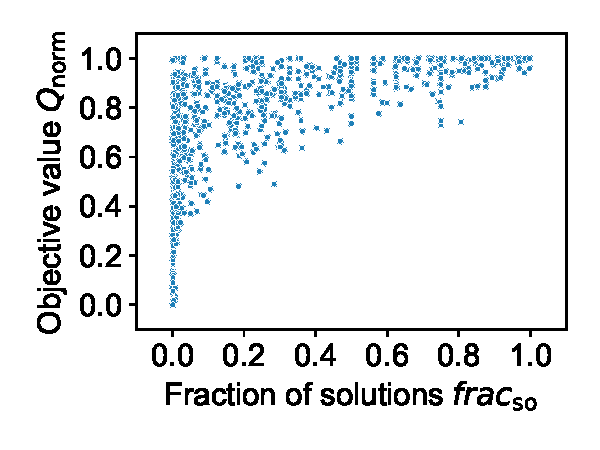
\includegraphics[width=0.95\textwidth, trim={0 15 0 10}, clip]{plots/syn-solutions-vs-objective.pdf}
			%JB: normalization of number of solutions: divide by total number of solutions (2 ^{number of features})
			%JB: clear correlation between size of solution space and objective (this trade-off is expected)
			%JB: even if solution space narrowed down significantly, high objective possible (the inverse does not hold)
			%JB: but existence of sweet spots naturally depends on dataset (how feature quality distributed)
			%JB: huge differences of individual evaluation metrics between constraint types
			%JB: weaker correlation if not taking size of solution space, but a cheaper proxy like number of constraints or number of constrained features
			%JB: note that we show objective of filter FS here; only weak to moderate correlation between number of solutions and prediction performance
		\end{subfigure}
	\end{figure}
	\centering
	$\mathit{frac}_{\text{se}} = \frac{\sum_{j=1}^{n} s_j}{n}$ \quad \vline \quad $Q_{\text{norm}} = \frac{\sum_{j=1}^{n} s_j  \cdot q(X_{\cdot{}j},y)}{\sum_{j=1}^{n} q(X_{\cdot{}j},y)}$ \quad \vline \quad $\mathit{frac}_{\text{so}} = \frac{\sum_{s \in \{0,1\}^n} \underset{c \in C}{\min}~c(s)}{2^n}$
\end{frame}

\section{Alternative Feature Selection}

\begin{frame}[t]{(C3) Alternative Feature Selection -- Approach}
	%JB: study for (C1) evaluated randomly generated constraints
	%JB: study for (C2) evaluated constraints based on domain knowledge
	%JB: - for time reasons, we don't discuss details
	%JB: - insight: Differently composed feature sets can yield similar feature-set quality
	\begin{itemize}
		\item Idea: Find feature sets optimizing feature-set quality while differing from each other
		%JB: using a set dissimilarity measure (in our case: Dice dissimilarity)
		\begin{itemize}
			\item Domain-independent constraint type
			\item Orthogonal to choice of feature-selection method
			%JB: we discuss integration into various methods
			\item Sequential or simultaneous search
			\item Number of alternatives~$a \in \mathbb{N}_0$ and feature-set dissimilarity threshold $\tau \in [0,1]$ as user parameters
		\end{itemize}
	\end{itemize}
	\pause
	\begin{columns}
		\column[t]{0.35\textwidth}
		\begin{greenblock}{Sequential-search problem}
			\vspace{-\baselineskip}
			\begin{equation*}
				\begin{aligned}
					\max_s &\quad Q(s,X,y) \\
					\text{subject to:} &\quad \forall F' \in \mathbb{F}:~d(F_s,F') \geq \tau
				\end{aligned}
				\label{eq:afs:afs-sequential}
			\end{equation*}
			%JB: alternatives found one by one, i.e., optimize quality of one feature set
			%JB: set of feature sets given, new alternative should differ from each
			%JB: optimization problem solved repeatedly
		\end{greenblock}
		\column[t]{0.6\textwidth}
		\begin{greenblock}{Simultaneous-search problem}
			\vspace{-\baselineskip}
			\begin{equation*}
				\begin{aligned}
					\max_{s^{(0)}, \dots, s^{(a)}} &\quad \operatorname*{agg}_{l \in \{0, \dots, a\}} Q(s^{(l)},X,y) \\
					\text{subject to:} &\quad \forall l_1, l_2 \in \{0, \dots, a\},~l_1 \neq l_2:~d(F_{s^{(l_1)}},F_{s^{(l_2)}}) \geq \tau
				\end{aligned}
				\label{eq:afs:afs-simultaneous}
			\end{equation*}
			%JB: all alternatives found at once
			%JB: still pairwise dissimilarity enforced
			%JB: examples for "agg": sum, min (latter balances qualities better)
		\end{greenblock}
	\end{columns}
	\pause
	\vspace{\baselineskip}
	\begin{itemize}
		\item Used dissimilarity measure: $d_{\text{Dice}}(F',F'') = 1 - \frac{2 \cdot |F' \cap F''|}{|F'| + |F''|} = 1 - \frac{2 \cdot \sum_{j=1}^n s'_j \cdot s''_j}{\sum_{j=1}^n s'_j + \sum_{j=1}^n s''_j}$
		%JB: remember that we use binary selection variables "s_j", which form vector "s" for each feature set
		%JB: for fixed feature-set sizes, resulting constraint becomes linear (in sequential search) or can easily be linearized (in simultaneous search)
	\end{itemize}
\end{frame}

\begin{frame}[t]{(C3) Alternative Feature Selection -- Complexity}
	\begin{itemize}
		\item Alternative feature selection is $\mathcal{NP}$-complete if:
		\begin{itemize}
			\item Simultaneous search with minimum as aggregation operator $\text{agg}(\cdot)$
			\item Linear notion of feature-set quality: $Q(s,X,y) = \sum_{j=1}^{n} q_j \cdot s_j$
			%JB: arguably simplest objective, also used in studies (C1) and (C2)
			\item No feature-set overlap ($\tau = 1$)
			\item Complete partitioning (each feature part of exactly one feature set)
			%JB: all features part of exactly one set
		\end{itemize}
		\pause
		\item Proof: Known as \textsc{Multi-Way Number Partitioning}~\cite{korf2010objective} or \textsc{Multiprocessor Scheduling}~\cite{garey2003computers} \qed
		%JB: if "k" bounded, problem known as "Balanced Number Partitioning" / "K-Partitioning"
		%JB: NP-hardness naturally transfers to more general problems
		\pause
		\vspace{\baselineskip}
		\item Further complexity-related contributions and results:
		\begin{itemize}
			\item Prove $\mathcal{NP}$-hardness for incomplete partitioning and feature-set overlap
			%JB: drop two of the four assumptions above
			%JB: reduction from base case above (no overlap, complete partitioning)
			\pause
			\item Prove polynomial runtime for sum-aggregation and sequential search with remaining conditions from above
			\pause
			\item Develop two heuristic search methods with approximation guarantee
			%JB: guarantee is a constant-factor approximation
			%JB: conditions for guarantee: linear objective, unused features, Dice dissimilarity, fixed "k" for all sets
		\end{itemize}
	\end{itemize}
\end{frame}

\begin{frame}[t]{(C3) Alternative Feature Selection -- Empirical Results}
	\begin{figure}
		\centering
		\begin{subfigure}[t]{0.32\textwidth}
			\centering
			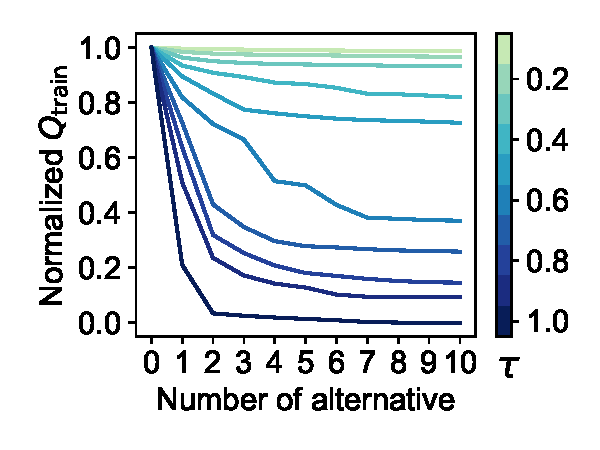
\includegraphics[width=\textwidth, trim={15 15 10 15}, clip]{plots/afs-impact-num-alternatives-tau-train-objective-max-fillna.pdf}
			\caption{Training-set objective value.}
		\end{subfigure}
		\hfill
		\begin{subfigure}[t]{0.32\textwidth}
			\centering
			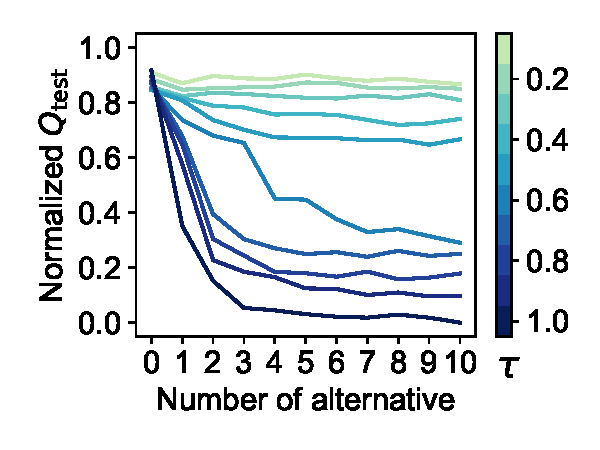
\includegraphics[width=\textwidth, trim={15 15 10 15}, clip]{plots/afs-impact-num-alternatives-tau-test-objective-max-fillna.pdf}
			\caption{Test-set objective value.}
		\end{subfigure}
		\hfill
		\begin{subfigure}[t]{0.32\textwidth}
			\centering
			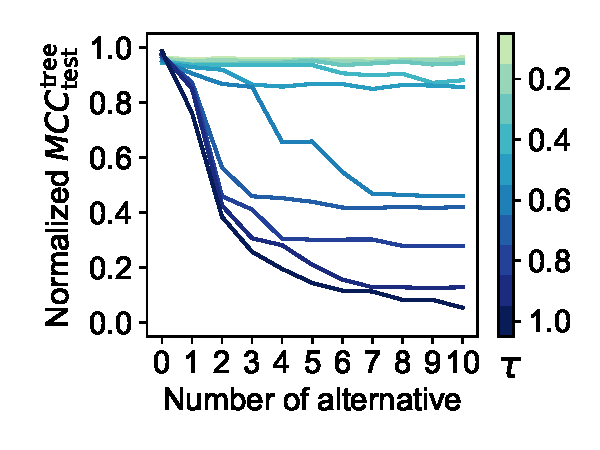
\includegraphics[width=\textwidth, trim={15 15 10 15}, clip]{plots/afs-impact-num-alternatives-tau-decision-tree-test-mcc-max-fillna.pdf}
			\caption{Test-set prediction performance.}
		\end{subfigure}
		\caption*{
			\normalsize Mean of feature-set quality, over the number of alternatives and dissimilarity threshold~$\tau$, by evaluation metric. % global caption-font-size setting not picked up here, so adjusted manually
			%JB: Results from sequential search with \emph{MI} as feature-selection method and $k=10$.
			%JB: Quality max-normalized per experimental setting, infeasible feature sets assigned a quality of~0.
		}
		%JB: here, one of five feature-set quality functions (an univariate objective), ten features to be selected, sequential search only
		%JB: three evaluation metrics, we take mean over datasets and cross-validation folds
		%JB: training-set objective value is 1 on 0th alternative due to max normalization (with sequential search run); decreases over number of alternatives, but strong dependecy on "tau", which makes sense (if feature sets have to be more dissimilar, less good features left)
		%JB: similar (but weaker) trend for other two metrics, but need not be 0 at a=0
	\end{figure}
\end{frame}

\section{Constrained Subgroup Discovery}

\begin{frame}[t]{(C4) Constrained Subgroup Discovery -- Approach}
	\begin{itemize}
		\item Subgroup discovery: ``Identifying descriptions of subsets of a dataset that show an interesting behavior''~\cite{atzmueller2015subgroup}
		%JB: `Descriptions of subsets': E.g., restrict ranges of numerical features or select particular values of categorical features
		%JB: unlike typical ML prediction models, need not cover full dataset with one subgroup
		%JB: Kind of extension to feature selection (one binary decision for each feature; now values play a role)
		%JB: `Interesting': Based on quality criterion, e.g., (relative) frequency of one particular class label
		\pause
		\vspace{\baselineskip}
		\item Scope: Binary classification with real-valued features
		\begin{itemize}
			\item Tabular dataset $X \in \mathbb{R}^{m \times n}$ (data objects $\times$ features)
			%JB: there also are variants of subgroup discovery that are more like frequent itemset mining, with binary feature values and only value 1 used in subgroup descriptions
			\item Prediction target $y \in \{0, 1\}^m$ (`interesting'/`positive' = 1)
			%JB: in regression, interestingness could refer to low or high values of target
			\pause
			\item Subgroup quality: Weighted Relative Accuracy
			\begin{itemize}
				\item $\text{WRACC} = \frac{m_b}{m} \cdot \left( \frac{m_b^+}{m_b} - \frac{m^+}{m} \right)$~\cite{lavravc1999rule}
				%JB: first factor is subgroup size, second is relative accuracy (precision in subgroup vs overall)
				\item \emph{+} $\leftrightarrow$ positive data object, \emph{b} $\leftrightarrow$ in subgroup (box)
			\end{itemize}
		\end{itemize}
		\pause
		\vspace{\baselineskip}
		\item Our goal: Improve interpretability with constraints
		%JB: on selected features
		\begin{itemize}
			\item Limit number of used features
			%JB: mainly discuss this constraint type in the following
			\item Find alternative subgroup descriptions
		\end{itemize}
	\end{itemize}
	\pause[0] % \visible or \onslide did not work, so we reset pause counter to show figure immediately
	\begin{tikzpicture}[remember picture,overlay]
		\node[xshift=-120pt,yshift=-140pt] at (current page.north east) {
			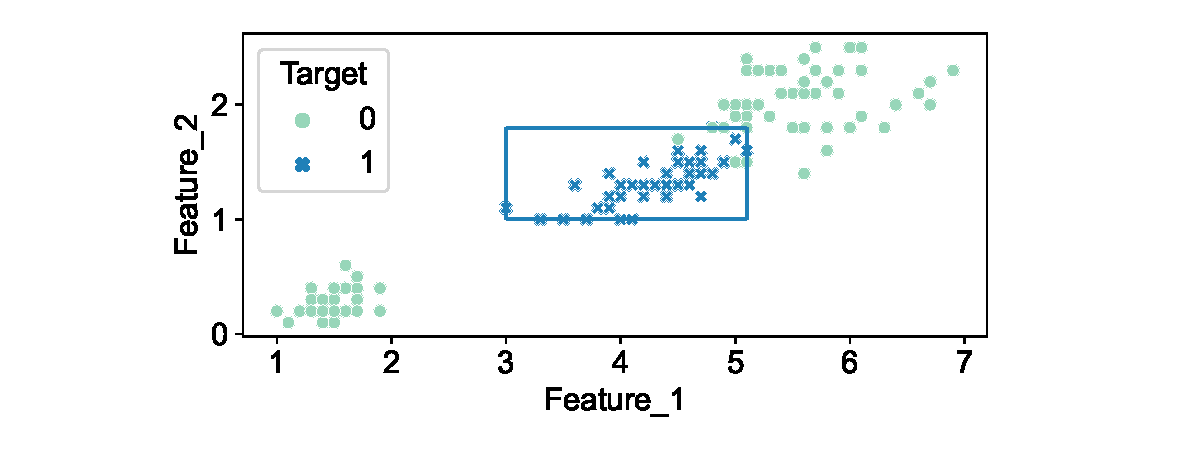
\includegraphics[width=0.45\textwidth, trim=80 15 100 15, clip]{plots/csd-exemplary-subgroup.pdf}
		};
	\end{tikzpicture}
\end{frame}

\begin{frame}[t]{(C4) Subgroup Discovery -- Formalization: Unconstrained}
	\vspace{-\baselineskip}
	%JB: contribution: SMT encoding for problem such that solver-based solution possible
	%JB: "unconstrained" in sense of no additional constraints apart from ones inherent in problem
	\begin{align*}
		\onslide<5->{
			\max &\quad & Q_{\text{WRAcc}} &= \frac{m_b^+}{m} - \frac{m_b \cdot m^+}{m^2} \tag*{(Objective: subgroup quality)} \\
			%JB: actually linar
		}
		\onslide<4->{
			\text{s.t.:} &\quad & m_b &:= \sum_{i=1}^{m} b_i \quad\text{and}\quad m_b^+ := \sum_{\substack{i \in \{1, \dots, m\} \\ y_i = 1 }} b_i \tag*{(Num of data objects in subgroup)} \\
		}
		\onslide<3->{
			&\quad \forall i \in \{1, \dots, m\} & b_i &\leftrightarrow \bigwedge_{j \in \{1, \dots, n\}} \left( \left( X_{ij} \geq \mathit{lb}_j \right) \land \left( X_{ij} \leq \mathit{ub}_j \right) \right) \tag*{(i-th data object in subgroup?)} \\
		}
		\onslide<2->{
			&\quad \forall j \in \{1, \dots, n\} & \mathit{lb}_j &\leq \mathit{ub}_j \tag*{(Constraint: relationship between bounds)} \\
			%JB: technically, you could even leave constraint out in most situations, as solutions with UB < LB would contain zero data objects in box and therefore have WRAcc = 0, while even a box containing only one positive data object (and nothing else) has a WRAcc > 0; however, if (1) feature values of all positive objects also exist with negative labels (no separation possible) and also there is no option to form an empty box (i.e., all combinations of feature values exist), or (2) there is a lower bound of number of instances covered, then best WRAcc may become < 0
		}
		\onslide<3->{
			&\quad & b &\in \{0, 1\}^m \tag*{(Auxiliary variables: subgroup membership)}  \\
			%JB: not strictly necessary (expressions above could be inlined), but I used variables in implemenentation (though not for m_b and m_b^+, which therefore have := in definition)
		}
		\onslide<1->{
			&\quad & \mathit{lb}, \mathit{ub} &\in \{\mathbb{R} \cup \{-\infty, +\infty\}\}^n \tag*{(Variables: lower/upper bounds of subgroup)}
		}
	\end{align*}
\end{frame}

\begin{frame}[t]{(C4) Subgroup Discovery -- Formalization: Cardinality}
	\begin{itemize}
		\item Concept: Limit number of features used (= selected) in subgroup description to $k \in \mathbb{N}$
		%JB: "k" is a user parameter
		\item Formally: Limit number of features whose bounds exclude at least one data object from subgroup
		%JB: i.e., technically, a feature appearing in subgroup description may still not be selected (cannot happen in our implementation because we post-process bounds of subgroups accordingly)
		\pause
		\vspace{0.5\baselineskip}
		\begin{equation*}
			\begin{aligned}
				\onslide<3->{
					\forall j \in \{1, \dots, n\}: && s^{\text{lb}}_j &\leftrightarrow \left( \mathit{lb}_j > \min_{i \in \{1, \dots, m\}} X_{ij} \right) \\
					\forall j \in \{1, \dots, n\}: &&s^{\text{ub}}_j &\leftrightarrow \left( \mathit{ub}_j < \max_{i \in \{1, \dots, m\}} X_{ij} \right) \\
					%JB: min and max feature values are constants here
				}
				\onslide<4->{
					\forall j \in \{1, \dots, n\}: && s_j &\leftrightarrow \left( s^{\text{lb}}_j \lor s^{\text{ub}}_j \right) \\
				}
				\onslide<5->{
					&& \sum_{j=1}^n s_j &\leq k \\
				}
				\onslide<2->{
					&& s, s^{\text{lb}}, s^{\text{ub}} &\in \{0, 1\}^n \\
					%JB: like b_i, these variables are not strictly necessary (could be inlined) but our implementation uses them
				}
			\end{aligned}
		\end{equation*}
	\end{itemize}
\end{frame}

\begin{frame}[t]{(C4) Constrained Subgroup Discovery -- Empirical Results}
	%JB: conduct four different kinds of experiments
	\begin{figure}
		\centering
		\begin{subfigure}[t]{0.32\textwidth}
			\centering
			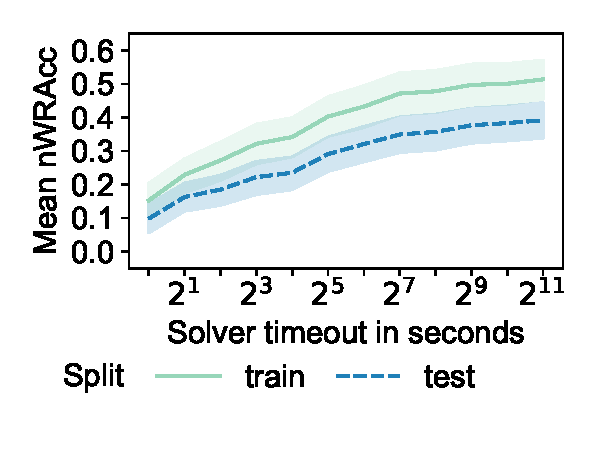
\includegraphics[width=\textwidth, trim={15 -27 15 15}, clip]{plots/csd-timeouts-nwracc.pdf} % actual bottom trimming should be different, but we use a negative number to manually top-align the figures (instead of only the captions)
			\caption*{Mean subgroup quality over solver timeouts for \emph{SMT} search.}
			%JB: without a feature-cardinality constraint
			%JB: for solver-based search we propose, one can vary timeout
			%JB: increase of subgroup-quality with timeout, and decreasing marginal gain (note logarithmic x-axis)
		\end{subfigure}
		\hfill
		\pause
		\begin{subfigure}[t]{0.32\textwidth}
			\centering
			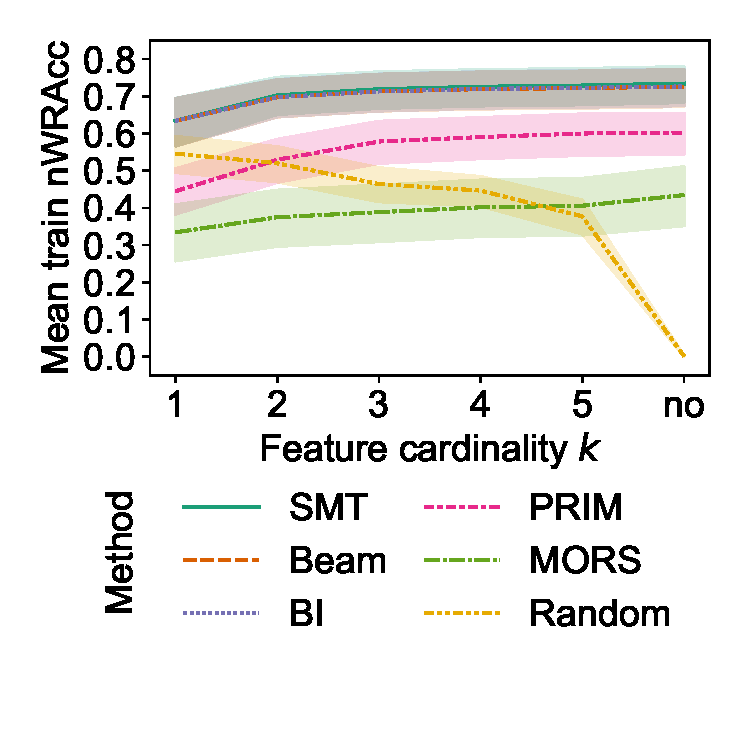
\includegraphics[width=\textwidth, trim={15 50 15 18}, clip]{plots/csd-cardinality-train-nwracc-no-timeout-datasets.pdf}
			\caption*{Mean training-set subgroup quality over feature-cardinality threshold~$k$.}
			%JB: only datasets without solver timeouts
			%JB: 95% confidence intervals based on datasets and cross-validation folds
			%JB: six SD methods and six feature-cardinality thresholds
			%JB: heuristics "Beam" and "BI" very close to exact optimum (interesting)
			%JB: increase of subgroup quality over "k" is small, i.e., small subgroup descriptions already yield high quality
		\end{subfigure}
		\hfill
		\pause
		\begin{subfigure}[t]{0.32\textwidth}
			\centering
			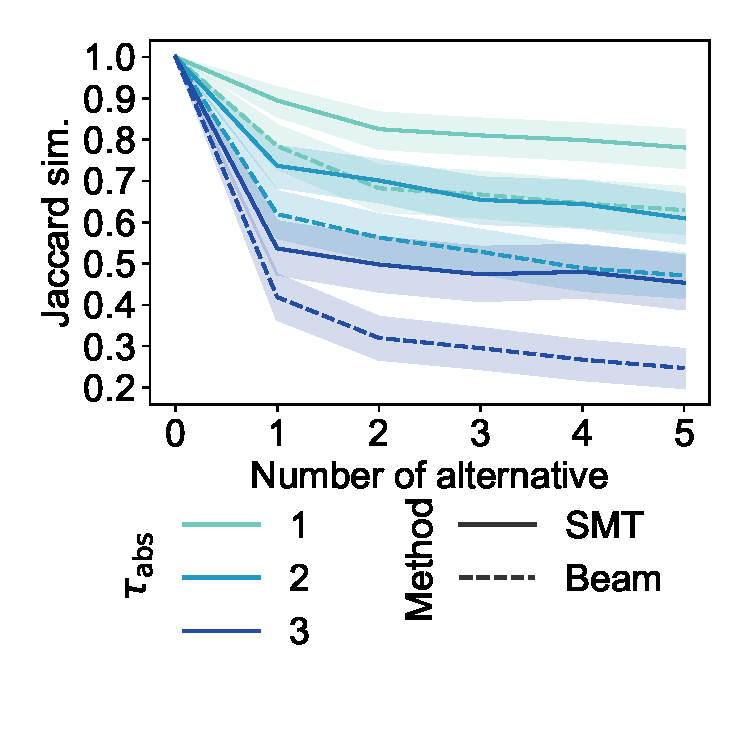
\includegraphics[width=\textwidth, trim={15 50 15 18}, clip]{plots/csd-alternatives-jaccard.pdf}
			\caption*{Mean similarity of alternative subgroup descriptions.}
			%JB: over the number of alternatives, by subgroup-discovery method and dissimilarity threshold~$\tau_{\text{abs}}$
			%JB: two SD methods, parameters for alternatives varied
			%JB: alternative subgroup descriptions less (data-object) similar to original the more alternatives desired and the higher (feature-selection) dissimilarity threshold (similar to AFS)
			%JB: similar trend for subgroup quality
		\end{subfigure}
	\end{figure}
\end{frame}

\section{Conclusion}

\begin{frame}[t]{Conclusions}
	\begin{itemize}
		\item Research gaps -- Most existing methods for feature selection and subgroup discovery:
		\begin{itemize}
			\item Do not consider domain knowledge
			\item Return only one solution, no alternatives
		\end{itemize}
		\pause
		\vspace{\baselineskip}
		\item Approach: Address both research gaps with constraints on selected feature sets
		\pause
		\vspace{\baselineskip}
		\item Core contributions:
		\begin{itemize}
			\item (C1) Evaluating the impact of constraints: \textcite{bach2022empirical}
			\item (C2) Using constraints to formulate scientific hypotheses: \textcite{bach2022empirical}
			\item (C3) Using constraints for alternative feature sets: \textcite{bach2023finding}, \textcite{bach2024alternative}
			\item (C4) Using constraints for feature selection in subgroup discovery: Bach (2025) \cite{bach2025subgroup}, \textcite{bach2024using} % first reference in this line doesn't have year (is included in "howpublished"), so we manually cite it
		\end{itemize}
		\item All code and data available online
	\end{itemize}
\end{frame}

\appendix
\beginbackup % subsequent slides do not impact overall slide count

\begin{frame}[plain]
	\centering
	\Huge Appendix
\end{frame}

\section{Appendix}

\begin{frame}[t]{Details of Underlying Publications}
	\begin{itemize}
		\item Constrained feature selection (\hyperlink{slide:contributions}{C1} and \hyperlink{slide:contributions}{C2}):
		\begin{itemize}
			\item \fullcite{bach2022empirical}
		\end{itemize}
		\item Alternative feature selection (\hyperlink{slide:contributions}{C3}):
		\begin{itemize}
			\item \fullcite{bach2023finding}
			\item \fullcite{bach2024alternative}
		\end{itemize}
		\item Constrained subgroup discovery (\hyperlink{slide:contributions}{C4}):
		\begin{itemize}
			\item \fullcite{bach2024using}
			\item \fullcite{bach2025subgroup}
		\end{itemize}
	\end{itemize}
\end{frame}

\begin{frame}[t]{Related Work}
	%JB: only small selection of related work discussed in dissertation
	\begin{itemize}
		\item Integrating domain knowledge and constraints:
		\begin{itemize}
			\item Feature selection: Typically only combination of one constraint type (like cost~\cite{paclik2002feature, plasberg2009feature}, cardinality~\cite{khushaba2011feature, yang2015budget}, or group~\cite{jacob2009group, yuan2006model}) and feature-selection method; exceptions (wrapper methods with black-box constraints):~\cite{groves2015toward, neutatz2021enforcing}
			%JB: Groves (2015) ignores invalid feature sets in four wrapper FS methods (no white-box solver), uses narrow set of constraint types (related to hierarchical feature grouping and temporal lags)
			%JB: Neutatz (2021) works with black-box constraints that mostly relate to whole ML system (acuuracy, fairness, training time, etc.) rather than feature selection per se (except number of selected features) and are checked after training/evaluation
			%JB: other notions of "constrained feature selection" include semi-supervised learning (constraints related to data objects) and Bayesian network learning (conditional independence constraints, learned and propagated automatically)
			\item Subgroup discovery: White-box formulations of different problem definitions~\cite{eckstein2002maximum, louveaux2014combinatorial} and integration of constraints into algorithmic search methods~\cite{atzmueller2005exploiting, meeng2021real}
			%JB: other white-box formulations use different constraint types, are CP or MIP (but not SMT), and do not compare against heuristics
			%JB: Maximum Box Problem (Eckstein 2002): capture as many positives as possible but no negatives
			%JB: Box Search Problem (Louveaux 2014): optimize sum of target variable of subgroup members (where target is continuous and can be negative)
			%JB: some SD methods use automatic quality-based pruning during search, but that approach differs from user constraints
			%JB: typical constraint types according to Meeng (2021): LB on quality, LB on members, UB on search depth
			%JB: studies on feature-cardinality constraint typically limited to one SD method or one cardinality threshold
			\item Other fields: E.g., AutoML~\cite{neutatz2023automl}, clustering~\cite{dao2024review}, pattern mining~\cite{silva2016constrained}, XAI~\cite{deutch2019constraints}; outside ML: software engineering~\cite{galindo2019automated}
			%JB: in ML, different problem definitions; software engineering has technically same problem as we (depending on objective function) but different domain/interpretation; technically, they often combine algorithm with sat solving, but pure white-box approach exist as well
		\end{itemize}
		\vspace{\baselineskip}
		\item Finding alternative solutions:
		\begin{itemize}
			\item Feature selection: Approaches that offer less user control over alternatives, e.g., ensemble feature selection~\cite{guru2018alternative, shekar2017diverse} or statistically equivalent feature sets~\cite{borboudakis2021extending, lagani2017feature}
			%JB: generally, less user control: in particular, no dissimilarity threshold
			%JB: ensemble feature selection: diversity may be sub-goal, but should "only" increase prediction performance in end (composition of feature sets is not of interest per se)
			%JB: statistically equivalent feature sets: no control over number, no redundancy at all, statistically equivalent for predictions, while we allow degradation of prediction performance and feature-set overlap (more flexible)
			\item Subgroup discovery: Subgroup-set selection~\cite{lucas2018ssdp+, proencca2022robust}; different problem definitions of alternative descriptions, e.g., description-based subgroup selection~\cite{leeuwen2012diverse} or equivalent subgroup descriptions of minimal length~\cite{boley2009non}
			%JB: subgroup-set selection wants to minimize rather than maximize overlap of data objects, and does not care about feature selection
			%JB: besides simultaneous search for diverse subgroups, also covering (exclude previously covered data objects), weighting, resampling, and post-processing approaches
			%JB: Leeuwen (2012) proposes 6 strategies for subgroup diversity, two related to descriptions, both integrated into simultaneous beam search, both offers less control than we do: (1) exclude descriptions with same quality and one condition less; (2) global bound on how often each feature selected in subgroup set
			%JB: Boley (2009): cover exactly same data objects with subset of given features; two search algorithms (not solver-based); inspired our NP-hardness proof
			\item Other fields: E.g., clustering~\cite{bailey2014alternative}, number partitioning~\cite{lawrinenko2017identical}, subspace search~\cite{fouche2021efficient}, XAI~\cite{mothilal2020explaining}
			%JB: problem definitions differ from ours (objective, constraints for alternatives)
			%JB: XAI example: counterfactuals should have different prediction outcome (rather than similar prediction quality) but similar feature values (rather than different feature selection)
		\end{itemize}
	\end{itemize}
\end{frame}

\begin{frame}[t]{Future Work}
	%JB: dissertation contains more ideas
	\begin{itemize}
		\item Different areas/directions: ML methodology, applied ML, and complexity theory
		%JB: results in one of these areas may be not that interesting for researchers from other areas
		\vspace{\baselineskip}
		\item ML methodology:
		\begin{itemize}
			\item Integrating constraints into more methods
			%JB: for FS, we focused on filter methods / white-box solving; only one wrapper, no embedded method
			\item Soft constraints
			%JB: may be violated; multi-objective problem, where solutions from Pareto front may be shown to user, or trade-off parameter
			\item Feature engineering
			%JB: could develop constraints for feature-creation operators, and/or consider constraint in automated feature engineering
		\end{itemize}
		\item Applied ML:
		\begin{itemize}
			\item Case studies with qualitative interpretation of results
			%JB: our interpretation is quantitative
			\item User-friendly systems
			%JB: we have Python packages (friendly for ML experts), but no interface for end users
		\end{itemize}
		\item Complexity theory:
		%JB: also further work regarding NP-hardness possible, e.g., objectives in AFS and feature-set overlap in ASDD
		\begin{itemize}
			\item Approximation complexity
			%JB: rather loose results (APX membership) for one quality function in AFS, no results in SD (though heuristic methods strong there as well)
			\item Parameterized complexity
			%JB: rather loose results at moment (XP membership), may be narrowed down
		\end{itemize}
	\end{itemize}
\end{frame}

\begin{frame}[t]{(C2) Scientific Hypotheses as Constraints -- Approach}
	\begin{itemize}
		\item Case study on impact of constraints in a specific use case
		\begin{itemize}
			\item Scenario~\cite{sudmanns2020data} from materials science: Predict density of dislocation reactions in a specimen under load
			%JB: Tensile test with aluminum specimen (could also be other face-centered cubic crystal)
			%JB: Dislocations (defects in material) appear and move as specimen deforms; reaction desnity should be predicted from other physical quantities
			%JB: Size of (5 micrometers)^3, partitioned into 5^3 voxels
			%JB: 22 time steps with intervals of ~ 5 ns
			\item Constraints express preferences regarding feature sets and hypotheses from domain
			%JB: preferences: global cardinality, inter-correlation, quality filter
			\item Idea: Hypotheses inconsistent to data should lower prediction quality significantly
		\end{itemize}
		\vspace{\baselineskip}
		\item Experimental design:
		\begin{itemize}
			\item One dataset with 14,903 data objects, 135 features, and continuous target
			\item Linear objective using Pearson correlation as $q(\cdot)$, four prediction models
			\item Constraint types: Three domain-independent (preferences) and twelve domain-specific (hypotheses)
		\end{itemize}
		\vspace{0.5\baselineskip}
		\begin{example}[Constraint type]
			$\text{Aggregate-or-original}(\{s_1, \dots, s_n\}) = \bigwedge_{p \in P} \left( \left( \bigvee_{a \in A} s_{(p,a)} \right) + \left( \bigvee_{l \in \{1, \dots, 12\}} s_{(p,l)} \right) \leq 1 \right)$\\
			$\leftrightarrow$ ``For each physical quantity $p$, do not select aggregate features $a$ and original features $l$ at the same time.'' %JB: original features measured in 12 directions (slip systems)
		\end{example}
	\end{itemize}
\end{frame}

\begin{frame}[t]{(C2) Scientific Hypotheses as Constraints -- Results}
	\begin{figure}
		\centering
		\begin{subfigure}{0.48\textwidth}
			\centering
			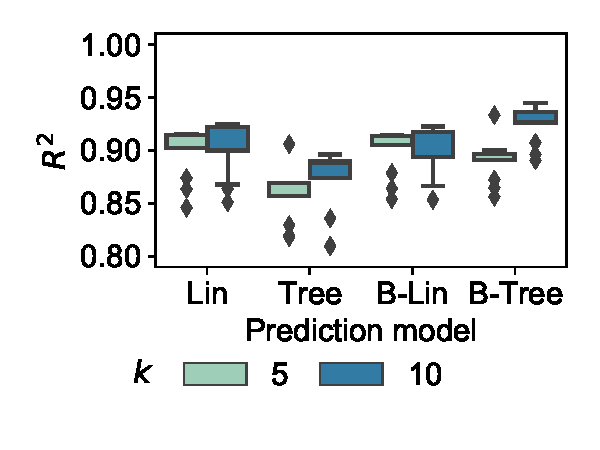
\includegraphics[width=\textwidth, trim={0 20 0 15}, clip]{plots/ms-prediction-performance-cardinality.pdf}
			\caption*{Distribution of prediction quality over constraint types (which express scientific hypotheses).}
			%JB: performance for k=5 comparable to k=10, and even simple linear regression good (feature selection makes sense in scenario)
			%JB: not much difference of prediction performance between constraint types -> cannot invalidate hypotheses
			%JB: similar observations as for prediction performance also for objective value
		\end{subfigure}
		\hfill
		\begin{subfigure}{0.48\textwidth}
			\centering
			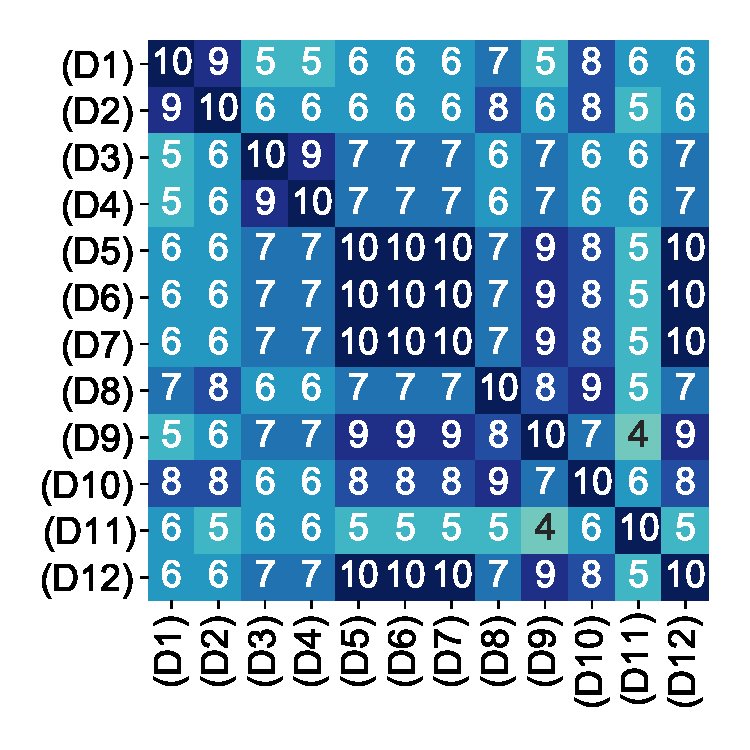
\includegraphics[width=0.7\textwidth, trim={0 20 0 15}, clip]{plots/ms-selected-similarity-card10.pdf}
			\caption*{Overlap size of feature sets between constraint types (for selecting $k=10$ features).}
			%JB: event though prediction performance similar, feature sets might differ -> interesting alternatives
			%JB: still, quite often results similar to UNCONSTRAINED (D12) -> constraints might not affect top features or top feature set might already satisfy constraints -> iterating with domain experts probably better
			%JB: selected features made sense to domain experts, mostly related to dislocation density
		\end{subfigure}
	\end{figure}
\end{frame}

\begin{frame}[t]{(C3) Alternative Feature Selection -- Experimental Design}
	\begin{itemize}
		\item 30 binary-classification datasets (with 106--9822 data objects and 15--168 features) from \emph{PMLB}~\cite{olson2017pmlb, romano2021pmlb}
		\item Five feature-set quality measures as objective functions
		%JB: From different categories: univariate filter (MI), multivariate filter (FCBF/mRMR), wrapper, and post-hoc importance
		\item Different search configurations for alternatives:
		\begin{itemize}
			\item Number of alternatives~$a$
			%JB: 10 for sequential search, up to 5 for simultaneous search
			\item Dissimilarity threshold~$\tau$
			%JB: all distinct values for k=5 and k=10
			\item Search methods (three solver-based, two heuristics)
		\end{itemize}
		\item Evaluation metrics:
		\begin{itemize}
			\item Objective value
			\item Prediction performance (MCC~\cite{matthews1975comparison})
			%JB: first two items quantify feature-set quality
			\item Runtime
			\item Optimization status
		\end{itemize}
		%JB: predictions with decision tree~\cite{breiman1984classification} and random forest~\cite{breiman2001random}; embedded approaches, so they also select features (which is not bad for us, we mainly want to limit input feature set and don't care what model does)
		\item \emph{SCIP}~\cite{bestuzheva2021scip} (a MIP solver) via {Google OR-Tools}~\cite{perron2022or-tools} as optimizer for solver-based search
		%JB: set timeout of 60 s, which affects 16% of feature sets in results
	\end{itemize}
\end{frame}

\begin{frame}[t]{(C4) Subgroup Discovery -- Formalization: Alternatives}
	\begin{itemize}
		\item Concept: Cover similar set of data objects as given subgroup with different set of selected features
		\begin{itemize}
			\item Repeat sequentially to get $a \in \mathbb{N}$ alternatives for dissimilarity threshold~$\tau \in \mathbb{R}_{\geq 0}$
			%JB: in my work on alternative feature selection, same user parameters
		\end{itemize}
		\vspace{\baselineskip}
		\item Chosen optimization objective: Maximize normalized Hamming similarity (= prediction accuracy)
		%JB: new objective! don't optimize subgroup quality anymore
		\begin{equation*}
			\text{sim}_{\text{nHamm}}(b^{(a)}, b^{(0)}) = \frac{1}{m} \cdot \sum_{i=1}^m \left( b_i^{(a)} \leftrightarrow b_i^{(0)} \right) = \frac{1}{m} \cdot \Big( \sum\limits_{\substack{i \in \{1, \dots, m\} \\ b_i^{(0)} = 1}} b_i^{(a)} + \sum\limits_{\substack{i \in \{1, \dots, m\} \\ b_i^{(0)} = 0}} \lnot b_i^{(a)} \Big)
			%JB: reminder: b_i denotes whether data object in subgroup or not
			%JB: (0) is orignal subgroup, (a) the alternative
			%JB: is linear (logical NOT can be linearized easily), while Jaccard similarity is not
		\end{equation*}
		\item Chosen dissimilarity constraints: From each existing feature set, deselect at least $\tau_{\text{abs}} \in \mathbb{N}$ (but $\leq k$) features
		%JB: "deselect": do not select again
		\begin{equation*}
			\forall l \in \{0, \dots, a-1\}:~ \text{dis}_{\text{des}}(s^{(a)}, s^{(l)}) = \sum_{\substack{j \in \{1, \dots, n\} \\ s^{(l)}_j = 1}} \lnot s^{(a)}_j \geq \min \left( \tau_{\text{abs}},~k^{(l)} \right)
			%JB: min prevents infeasibility
			%JB: not a commonly used measure, not even symmetric
			%JB: however, linear and antimonotonic (Dice and Jaccard are not), which eases integration into solver and heuristics
		\end{equation*}
		%JB: other constraints from subgroup discovery remain in problem as is
	\end{itemize}
\end{frame}

\begin{frame}[t]{(C4) Subgroup Discovery -- Complexity}
	\begin{itemize}
		\item Subgroup discovery with a feature-cardinality constraint is $\mathcal{NP}$-complete
		\item Proof: Reduction from \textsc{Set Covering}~\cite{karp1972reducibility}
		\begin{itemize}
			\item Original problem: Given set of elements~$E = \{e_1, \dots, e_m\}$, set of sets~$\mathbb{S} = \{S_1,  \dots, S_n\}$ with $E = \bigcup_{S \in \mathbb{S}} S$, and a cardinality~$k \in \mathbb{N}$, does subset $\mathbb{C} \subseteq \mathbb{S}$ with $|\mathbb{C}| \leq k$ and $E = \bigcup_{S \in \mathbb{C}} S$ exist?
			\item Perfect-subgroup discovery: Find subgroup containing all positive data objects ($y_i = 1$) and zero negatives ($y_i = 0$)
			%JB: may not exist, i.e., search problem instead of optimization problem
			\item Problem transformation:
			%JB: from set covering to perfect-subgroup discovery
			\begin{itemize}
				\item Dataset~$X \in \{0, 1\}^{(m + 1) \times n}$ with $X_{ij} := (e_i \in S_j)$
				%JB: elements become data objects, sets become features, set membership becomes feature value
				%JB: binary is special case of real-valued
				\item Data Object $m+1$ represents element not contained in any set, i.e., $X_{(m+1)j} = 0$
				\item Prediction target $y \in \{0, 1\}^{m+1}$ with $y_{m+1} = 1$ and $y_i = 0$ otherwise
				%JB: indicates whether not contained in any set
				%JB: further, parameter "k" remains as-is
			\end{itemize}
			\item Perfect subgroup only contains Data Object $m+1$ and uses $\mathit{lb}_j = \mathit{ub}_j = 0$ conditions for selected features
			%JB: new data object only has 0 as feature values
			%JB: bounds [0, 1] represent unselected features
			\item Other data objects have value 1 for at least one selected feature $\rightarrow$ each element is in a selected set
			\item I.e., algorithm for perfect-subgroup discovery also solves \textsc{Set Covering}
			%JB: however, latter is NP-hard, so former is NP-hard as well (and NP-complete since in NP)
			\item Optimizing subgroup quality typically at least as hard as finding perfect subgroup
			%JB: depends on notion of subgroup quality
		\end{itemize}
	\end{itemize}
\end{frame}

\begin{frame}[t]{(C4) Subgroup Discovery -- Experimental Design}
	\begin{itemize}
		\item 27 binary-classification datasets (with 106--9822 data objects and 20--168 features) from \emph{PMLB}~\cite{olson2017pmlb, romano2021pmlb}
		\item Six subgroup-discovery methods:
		\begin{itemize}
			\item Solver-based (novel): \emph{SMT} (using \emph{Z3}~\cite{bjorner2015nuz, deMoura2008z3} as optimizer)
			\item Heuristics (related work): \emph{Beam}, \emph{BI}~\cite{mampaey2012efficient}, \emph{PRIM}~\cite{friedman1999bump}
			%JB: iteratively and greedily restrict the subgroup's bounds, with one feature per iteration (PRIM: prune fixed fraction of data objects; Beam/BI: test all possible cuts)
			\item Baselines (novel): \emph{MORS} (Minimal Optimal Recall Subgroup), \emph{Random}
			%JB: MORS -- minimal bounds such that all positive data objects are in subgroup (exclude as many negative data objects as possible); will play a bigger role in PhD Colloquium on complexity
			%JB: Random -- repeated random sampling of bounds
		\end{itemize}
		%JB: hyperparameters fixed for all methods
		\item Four experimental scenarios: Unconstrained, two constraint types, and solver timeouts
		%JB: in conference version, only phrased as two scenarios (the two constraint types)
		\begin{itemize}
			\item Solver timeouts: \{1~s, 2~s, 4~s, $\dots$, 2048~s\}
			\item Feature-cardinality constraints: $k \in \{1, 2, 3, 4, 5\}$
			\item Alternative subgroup descriptions: $k=3$, $a=5$, and $\tau_{\text{abs}} \in \{1, 2, 3\}$
		\end{itemize}
		\item Evaluation metrics:
		\begin{itemize}
			\item Subgroup quality (nWRAcc~\cite{lavravc1999rule, mathonat2021anytime})
			\item Runtime
			\item For alternatives: Similarity~\cite{choi2010survey} (Normalized Hamming and Jaccard)
		\end{itemize}
		\item \emph{Z3}~\cite{bjorner2015nuz, deMoura2008z3} (an SMT solver) as optimizer for solver-based search
	\end{itemize}
\end{frame}

\begin{frame}[t, allowframebreaks]{References}
	\renewcommand*{\bibfont}{\small} % use a smaller font for bib than for main text
	\printbibliography
\end{frame}

\backupend

\end{document}
